\chapter{Anomalous Gauge Coupling Theory}
\label{chap:anomalousgaugecouplingtheory}

\chapterquote{There, sir! that is the perfection of vessels!}
{Jules Verne, 1828--1905}
%
%========================================================================================
%========================================================================================
%
\section{The Standard Model}
The Standard Model is a non-abelian gauge theory of the $\text{SU}(3) \times \text{SU}(2)_{\text{L}} \times \text{U}(1)$ symmetry group.  It provides a description of three of the four fundamental forces of nature: the electromagnetic, weak and strong nuclear forces \cite{Griffiths:1987tj,Peskin:1995ev}.  The Standard Model contains a total of 24 fermion fields: six flavours of quark, each with three colours, and six leptons.  A summary of the properties of these particles is given in table \ref{table:smleptons} and \ref{table:smquarks}.  As these fields are spin-$\frac{1}{2}$, they obey the Dirac equation:
%
\begin{equation}
\mathcal{L} = \overline{\psi}(i \slashed{\partial} - m)\psi \text{ ,}
\end{equation}
%
\noindent where $\mathcal{L}$ is the Lagrangian density and $m$ is a mass term.  The derivative term, $\slashed{\partial} = \gamma^{\mu}\partial_{\mu}$, represents a summation over the partial derivate, $\partial^{\mu} = (\frac{\partial}{\partial{t}},\frac{\partial}{\partial{x}},\frac{\partial}{\partial{y}},\frac{\partial}{\partial{z}})$, of the scalar field $\psi$ and the gamma matrices, $\gamma^{\mu}$.  Each of the gauge transformations of the Standard Model are defined by a unitary operator \textrm{U}, which acts to transform the vector space, $\Psi$, formed from a combination of fermion fields, $\psi$, in the following way:
%
\begin{equation}
\Psi \rightarrow \Psi' = \textrm{U}\Psi \text{ .}
\end{equation}
%
In the Standard Mode, the Lagrangian density describing the fermion fields is invariant under a $\text{SU}(3)$, a $\text{SU}(2)_{\text{L}}$ and a U(1) gauge transformations .  The $\text{SU}(2)_{L}$ gauge symmetry acts on doublets formed of pairs of left handed chiral components of the fermion fields, $\psi_{L} = \frac{1}{2}(1-\gamma_{5})\psi$, while the right handed components, $\psi_{R} = \frac{1}{2}(1+\gamma_{5})\psi$, transform trivially as a singlets.  Similarly, the SU(3) symmetry acts on triplets formed of the fermion fields for each flavour of quark.  All fields transform under the fundamental representation of U(1).  The invariance of the Standard Model Lagrangian to these gauge transformations is established by introducing 12 gauge fields, which are summarised in table \ref{table:smbosons}, via the covariant derivate of the fermion fields:
%
\begin{equation}
\partial^{\mu} \rightarrow D^{\mu} = \partial^{\mu} + ig_{1}YB^{\mu} + ig_{2} \textbf{T} \cdot \textbf{W}^{\mu} + ig_{3}\textbf{X} \cdot \textbf{G}^{\mu} \text{ ,}
\end{equation}
%
\noindent where $B^{\mu}$ is the gauge field for the U(1) symmetry, $\textbf{W}^{\mu}$ ($\text{W}^{\mu}_{j}, j =1,2,3$) are the fields of the $\text{SU}(2)_{\text{L}}$ symmetry and $\textbf{G}^{\mu}$ ($\text{G}^{\mu}_{j}, j =1,..,8$) are the fields of the SU(3).  $Y$ is the weak hypercharge, which is related to the chirality and flavour of the fermion it relates to.  $g_{1}$, $g_{2}$ and $g_{3}$ are three coupling constants related to the three symmetry groups of the Standard Model.  Mixing of the gauge fields for the U(1) and SU(2) symmetry of the form:
%
\begin{equation}
\text{Z}_{\mu} = \text{cos}{\theta_{W}} \text{W}^{3}_{\mu} - \text{sin}{\theta_{W}} \text{B}_{\mu} \text{ ,}\\
\text{A}_{\mu} = \text{sin}{\theta_{W}} \text{W}^{3}_{\mu} + \text{cos}{\theta_{W}} \text{B}_{\mu} \text{ ,}\\
\text{W}^{\pm}_{\mu} = \frac{1}{\sqrt{2}}(\text{W}^{1}_{\mu} \mp i \text{W}^{2}_{\mu}) \text{ ,}
\end{equation}
%
\noindent where:
%
\begin{equation}
\text{cos}{\theta_{W}} = \frac{g_{2}}{g_{1}+g_{2}} \text{ and } \text{sin}{\theta_{W}} = \frac{g_{1}}{g_{1}+g_{2}} \text{ ,}
\end{equation}
%
\noindent gives the electroweak gauge bosons; $\text{W}^{\pm}$, Z and $\gamma$.  This mixing ensures that the $\text{W}^{\pm}$ and Z bosons become massive, while the $\gamma$ remains massless.  The $\text{G}^{\mu}_{j}$ fields are the eight massless gluons of the strong force.   $\textbf{T}$ and $\textbf{X}$ are the generators for the SU(2) and SU(3) symmetries, which are typically chosen as:
%
\begin{equation}
T_{i} = \frac{1}{2}\tau_{i} \text{ ,} \\
X_{i} = \frac{1}{2}\lambda_{i} \text{ ,} \\
\end{equation}
%
\noindent where $\tau$ and $\lambda$ are the Pauli and the Gell-Mann matrices respectively.  

The gauge fields of the Standard Model, $B_{\mu}$, $\textbf{W}_{\mu}$ and $\textbf{G}_{\mu}$, transform under the gauge transformations as:
%
\begin{equation}
K_{\mu} \rightarrow K'_{\mu} = UK_{\mu}U^{\dagger} + \frac{i}{g}(\partial^{\mu}U)U^{\dagger} \text{ ,} 
\end{equation}
%
\noindent where $K_{\mu}$ is any of $B_{\mu}$, $\textbf{W}_{\mu}$ and $\textbf{G}_{\mu}$ and $g$ is the coupling constants associated to the relevant gauge field.  As the $B_{\mu}$, $\textbf{W}_{\mu}$ and $\textbf{G}_{\mu}$ gauge fields are spin-1, they are described by the Proca action:
%
\begin{equation}
\mathcal{L} = -\frac{1}{4}F^{{\mu}{\nu}}_{i}F_{{\mu}{\nu}{i}} + \frac{1}{2}m_{K}^{2}K_{i\mu}K^{\mu}_{i} \text{ ,} 
\end{equation}
%
\noindent where:
%
\begin{equation}
F^{{\mu}{\nu}}_{i} = \partial^{\mu}K^{\nu}_{i} - \partial^{\nu}K^{\mu}_{i} - gf_{ijk}K^{\mu}_{j}K^{\nu}_{k} \text{ ,} 
\end{equation}
%
\noindent where $f_{ijk}$ are the fully anti-symmetric structure constants of the group, $K^{\mu}_{i}$ is the $i^{th}$ gauge field of the group and $m_{K}$ is a mass term for the gauge boson.  The structure constants are defined from the commutation relations between generators of the symmetry group:
%
\begin{equation}
[T_{i},T_{j}] = if_{ijk}T_{k} \text{.} 
\end{equation}
%
\noindent These structure constants that govern the self-interactions for the gauge bosons.  There is only one structure constant for the U(1) symmetry, which is zero, as the U(1) symmetry is abelian.  The SU(2) symmetry structure constants are $f_{ijk} = \epsilon_{ijk}$, where $\epsilon_{ijk}$ is the Levi-Civita tensor.  Due to the symmetries that are present in the Standard Model, $m_{K} = 0$ for all the gauge fields, however, it is clear that is is not the case.  Therefore, to generate gauge boson mass terms a Higgs field is introduced that undergoes spontaneous symmetry breaking, as described in section \ref{sec:higgsphysics}. 

\begin{table}[h!]
\centering
\begin{tabular}{l l r r r}
\hline
Generation & Particle & Mass [MeV] & Spin & Q/e \\
\hline
1 & $e^{-}$ & $548.579909070\pm0.000000016$ & 1/2 & -1 \\
& $\nu_{e}$ & - & 1/2 & 0 \\
\hline
2 & $\mu^{-}$ & $105.6583745\pm0.0000024$ & 1/2 & -1 \\
& $\nu_{\mu}$ & - & 1/2 & 0 \\
\hline
3 & $\tau^{-}$ & $1776.86\pm0.12$ & 1/2 & -1 \\
& $\nu_{\tau}$ & - & 1/2 & 0 \\
\end{tabular}
\caption[The mass, spin and electric charge (Q) of the leptons found in the Standard Model \cite{Beringer:1900zz}.  Neutrino masses have not been included in the above table as precise measurements are yet to be made.  However, oscillations between different neutrino flavour states have been observed, which indicates that the flavour and mass eigenstates differ and that the neutrinos have a non-zero mass.  The current upper bound on neutrino mass measurements is 2 eV.]{The mass, spin and electric charge (Q) of the leptons found in the Standard Model \cite{Beringer:1900zz}.  Neutrino masses have not been included in the above table as precise measurements are yet to be made.  However, oscillations between different neutrino flavour states have been observed, which indicates that the flavour and mass eigenstates differ and that the neutrinos have a non-zero mass.  The current upper bound on neutrino mass measurements is 2 eV.}
\label{table:smleptons}
\end{table}

\begin{table}[h!]
\centering
\begin{tabular}{l l r r r}
\hline
Generation & Particle & Mass [MeV] & Spin & Q/e \\
\hline
1 & $u$ & $2.2^{+0.6}_{-0.4}$ & 1/2 & +2/3 \\
 & $d$ & $4.7^{+0.5}_{-0.4}$ & 1/2 & -1/3 \\
\hline
2 & $c$ & $1270\pm30$ & 1/2 & +2/3 \\
 & $s$ & $98^{+8}_{-4}$ & 1/2 & +2/3 \\
\hline
3 & $t$ & $173210 \pm 510 \pm 710$ & 1/2 & +2/3 \\
 & $b$ & $4180^{+40}_{-30}$ & 1/2 & -1/3 \\
\end{tabular}
\caption[The mass, spin and electric charge (Q) of the quarks found in the Standard Model \cite{Beringer:1900zz}.  Each of the particles in the above table corresponds to three fermion fields, one for each of the three colours of the SU(3) symmetry.]{The mass, spin and electric charge (Q) of the quarks found in the Standard Model \cite{Beringer:1900zz}.  Each of the particles in the above table corresponds to three fermion fields, one for each of the three colours of the SU(3) symmetry.} 
\label{table:smquarks}
\end{table}

\begin{table}[h!]
\centering
\begin{tabular}{l l r r r}
\hline
Force & Particle & Mass [GeV] & Spin & Q/e \\
\hline
Electromagnetic & $\gamma$ & 0 & 1 & 0 \\
\hline
Weak Nuclear & $\text{W}^{\pm}$ & $80.385 \pm 0.015$ & 1 & $\pm$ 1 \\
& Z & $91.1876 \pm 0.0021$ & 1 & 0 \\
\hline
Strong Nuclear & $g$ ($\times 8$ colours) & 0 & 1 & 0 \\
\hline
Higgs & H & $125.1 \pm 0.3$ & 0 & 0 \\
\end{tabular}
\caption[The mass, spin and electric charge (Q) of the gauge bosons found in the Standard Model \cite{Beringer:1900zz}.  The $\gamma$ and $g$s theoretically have zero mass, which is consistent with measurements.  The upper bound on the $\gamma$ mass has been measured at $10^{-18}$ eV, while gluon masses of up to a few MeV have not been precluded.  The upper bound on the magnitude of the charge of the $\gamma$ is measured at $10^{-35}$.]{The mass, spin and electric charge (Q) of the gauge bosons found in the Standard Model \cite{Beringer:1900zz}.  The $\gamma$ and $g$s theoretically have zero mass, which is consistent with measurements.  The upper bound on the $\gamma$ mass has been measured at $10^{-18}$ eV, while gluon masses of up to a few MeV have not been precluded.  The upper bound on the magnitude of the charge of the $\gamma$ is measured at $10^{-35}$.}
\label{table:smbosons}
\end{table}

%========================================================================================
%========================================================================================

\section{Higgs Physics}
\label{sec:higgsphysics}
Mass terms are generated in the Standard Model by introducing a Higgs field that undergoes spontaneous symmetry breaking.  This allows the gauge bosons, as well as the quarks and leptons, to obtain a mass, while still respecting the gauge symmetries found in the Standard Model.  

%========================================================================================

\subsection{Spontaneous Symmetry Breaking}
\label{sec:ssb}
To illustrate spontaneous symmetry breaking, consider a complex scalar field \psi with the Klein-Gordon Lagrangian:
%
\begin{equation}
\mathcal{L} = \partial^{\mu} \psi^{*} \partial_{\mu} \psi -m^{2} |\psi|^{2} = \partial^{\mu} \psi^{*} \partial_{\mu} \psi - V(\psi) \text{ ,}
\label{equ:kleingordon}
\end{equation}
%
\noindent where $\mathcal{L}$ the is Lorentz invariant Lagrangian density, $\partial^{\mu} = (\frac{\partial}{\partial{t}},\frac{\partial}{\partial{x}},\frac{\partial}{\partial{y}},\frac{\partial}{\partial{z}})$ is the partial derivative of the scalar field $\psi$, $m$ is a mass term and $V(\psi)$ is the potential the field $\psi$.  This Lagrangian density is invariant under the global symmetry $\psi \rightarrow e^{i\alpha} \psi$.  By adding extra terms to the Lagrangian, which retain the invariance to the global symmetry, it is possible to modify the interactions of this scalar field.  For example consider modifying the potential of the scalar field to the following:
%
\begin{equation}
\text{V}(\psi) = m^{2}|\psi|^{2} + \lambda |\psi|^{4} \text{ ,}
\end{equation}
%
\noindent If $m^{2} > 0$, the potential has a minima at zero, however, if $m^{2} < 0$ then the minima exists on a circle in the complex $\psi$ plane, which is centred at $(0,0)$ and has radius $v = \sqrt{-m^{2}/\lambda}$.  To quantise this theory it is necessary to expand about the minima of the potential.  However, in the case of $m^{2} < 0$ there are an infinite number of choices of minima to expand about.  Irrespective of the choice of minima used to expand the field about, the symmetry $\psi \rightarrow e^{i\alpha} \psi$ is broken.  Fluctuations about the minima along the degenerate direction leave the potential unchanged, which is a consequence of the breaking of the $\psi \rightarrow e^{i\alpha} \psi$ symmetry; this is known as spontaneous symmetry breaking.

Goldstone's theorem \cite{Goldstone:1962es} implies that for Lorentz-invariant theories spontaneous symmetry breaking always leads to the existence a massless particle.  For example, consider expanding the complex scalar $\psi$ one of the minimia:
%
\begin{equation}
\psi = \frac{1}{\sqrt{2}}(v + \psi_{1} + i \psi_{2}) \text{ ,}
\end{equation}
%
\noindent where $\psi_{1}$ and $\psi_{2}$ are real fields and $v = \sqrt{-m^{2}/\lambda}$.  Applying this parameterisation to the Lagrangian yields a mass term of $\sqrt{-m^{2}}$ for the $\psi_{1}$ field, however, there is no corresponding mass term for the $\psi_{2}$ field, which indicates that it is massless as predicated by Goldstone's theorem:
%
\begin{equation}
\mathcal{L} = \frac{1}{2}\partial^{\mu} \psi_{1} \partial_{\mu} \psi_{1} + \frac{1}{2}\partial^{\mu} \psi_{2} \partial_{\mu} \psi_{2} - m^{2}|\psi_{1}|^{2} + ... \text{ ,}
\end{equation}
%

Spontaneous symmetry breaking is the origin of the gauge boson mass terms when applied to local symmetries instead of global ones.  For example consider the global symmetry, $\psi \rightarrow e^{i\alpha} \psi$, that exists in equation \ref{equ:kleingordon}.  If this global symmetry is promoted to a local symmetry by letting $\alpha \rightarrow \alpha(x)$ and $\partial^{\mu} \rightarrow D^{\mu} = \partial^{\mu} + iA^{\mu}$, where $A^{\mu}$ a the gauge field that transforms as $A^{\mu} \rightarrow A^{\mu} - \partial^{\mu}\alpha(x)$, the Lagrangian in \ref{equ:kleingordon} becomes:
%
\begin{equation}
\mathcal{L} = (D^{\mu} \psi)^{*} (D_{\mu} \psi) - m^{2} |\psi|^{2} - \lambda |\psi|^{4} \text{ .}
\end{equation}
%
\noindent If there is a non-zero minima in the potential, i.e. $m^{2} < 0$ and $v = \sqrt{-m^{2}/\lambda}$, then a gauge boson mass term, $+\frac{v^{2}}{2} A^{\mu} A_{\mu}$, is present after spontaneous symmetry breaking.

%========================================================================================

\subsection{Electroweak Interactions}
\label{sec:ewint}
The electroweak sector of the Standard Model is that related to the $\text{SU}(2)_{\text{L}} \times \text{U}(1)$ symmetry \cite{Ellis:2013jnq}.  In this sector, spontaneous symmetry breaking must occur in such a way as to give three massive gauge bosons,  $\text{W}^{\pm}$ and Z, and one massless gauge boson, the $\gamma$.  This can be achieved through a Higgs field, H, that transforms as a doublet under the $\text{SU}(2)_{\text{L}}$ symmetry.  The Lagrangian for this field is:
%
\begin{equation}
\mathcal{L}_{Higgs} = (D_{\mu}\text{H})^{\dagger}D^{\mu}\text{H} - \text{V}(\text{H}) \text{ ,}
\end{equation}
%
\noindent where:
%
\begin{equation}
\text{V}(\text{H}) = -\mu^{2}\text{H}^{\dagger}\text{H} + \lambda (\text{H}^{\dagger}\text{H})^{2} \text{ ,}
\end{equation}
%
\noindent where $\mu$ and $\lambda$ are constants.  The covariant derivative of this Higgs field must satisfy the $\text{SU}(2)_{\text{L}} \times \text{U}(1)$ gauge symmetry meaning it takes the form:
%
\begin{equation}
D_{\mu} \text{H} = (\partial_{\mu} + ig_{1}YB_{\mu} + ig_{2}\frac{\tau^{i}}{2}W^{i}_{\mu})H \text{ ,}
\end{equation}
%
\noindent where $g_{1}$ and $g_{2}$ are coupling constants for the relevant gauge symmetries, $Y = \frac{1}{2}$ is the weak hypercharge of the Higgs, $\tau^{i}$ are the Pauli matrices and $B_{\mu}$ is the gauge field related to the U(1) symmetry and $W^{i}_{\mu}$ are the gauge fields related to the $\text{SU}(2)_{\text{L}}$ symmetry.  

Consider spontaneously breaking the symmetry in the Higgs sector by expanding the Higgs field about a non-zero vacuum expectation value (vev):
%
\begin{equation}
\langle \text{H} \rangle = \binom{0}{\frac{v}{\sqrt{2}}} \text{ ,}
\end{equation}
%
\noindent where the minima of the field is defined as:
%
\begin{equation}
\frac{v}{\sqrt{2}} = \sqrt{\frac{\mu^{2}}{2\lambda}} \text{ .}
\end{equation}
%
\noindent with $v$ being real.  In that case, the kinematic term in the Higgs Lagrangian, $D^{\mu} \text{H}^{\dagger} D{\mu} \text{H}$, contains mass terms for the gauge bosons.  If there is mixing of the $\text{SU}(2)_{\text{L}}$ and U(1) fields of the form:
%
\begin{equation}
\text{Z}_{\mu} = \text{cos}{\theta_{W}} \text{W}^{3}_{\mu} - \text{sin}{\theta_{W}} \text{B}_{\mu} \text{ ,}\\
\text{A}_{\mu} = \text{sin}{\theta_{W}} \text{W}^{3}_{\mu} + \text{cos}{\theta_{W}} \text{B}_{\mu} \text{ ,}\\
\text{W}^{\pm}_{\mu} = \frac{1}{\sqrt{2}}(\text{W}^{1}_{\mu} \mp i \text{W}^{2}_{\mu}) \text{ ,}
\end{equation}
%
\noindent then the gauge boson mass terms are:
%
\begin{equation}
\frac{(gv)^{2}}{4} \text{W}^{+}_{\mu} \text{W}^{-\mu} + \frac{(g^{2} + g'^{2})v^{2}}{8} \text{Z}_{\mu} \text{Z}^{\mu} \text{ .}\\
\end{equation}
%
\noindent This gives the gauge boson masses as:
%
\begin{equation}
\begin{aligned}
m_{\text{W}} = & \frac{gv}{2} \text{ ,} \\
m_{\text{Z}} = & \frac{v\sqrt{g^{2} + g'^{2}}}{2} = \frac{m_{W}}{\text{cos}{\theta_{W}}} \text{ ,} \\
m_{\text{A}} = & 0 \text{ ,}
\end{aligned}
\end{equation}
%
\noindent where $\theta_{W}$ is known as the Weinberg angle.  This mixing produces a massless gauge boson, the $\gamma$, and three massive gauge bosons, the $W^{\pm}$ and $Z$.  By acquiring a non-zero vev, the Higgs field breaks the $\text{SU}(2)_{\text{L}} \times \text{U}(1)$ symmetry that was present in the Lagrangian to the $\text{U}(1)_{em}$ symmetry of electromagnetism.  

The ratio of the masses of the $W^{\pm}$ and $Z$ bosons is predicted when spontaneously breaking the symmetry in the Higgs sector and crucially sets the $\rho$ parameter to be 1, where the $\rho$ parameter is defined as:
%
\begin{equation}
\rho = \frac{m_{\text{W}}^{2}}{m_{\text{Z}}^{2}\text{cos}{\theta_{W}}^{2}} = 1\text{ .}
\label{equ:custodialsymmetry}
\end{equation}
%
\noindent This is a consequence of the Higgs potential containing custodial symmetry \cite{Beringer:1900zz}.  As the $\rho$ parameter has been experimentally measured to be $1.00040 \pm 0.00024$ \cite{Agashe:2014kda}, it is clear that any extension to the Standard Model should retain this result.

%========================================================================================
%HERE
\subsubsection{Custodial Symmetry}
The Higgs Lagrangian:
%
\begin{equation}
\mathcal{L}_{Higgs} = (D_{\mu}\text{H})^{\dagger}D^{\mu}\text{H} - \text{V}(\text{H}) \\
\text{V}(\text{H}) = -\mu^{2}\text{H}^{\dagger}\text{H} + \lambda (\text{H}^{\dagger}\text{H})^{2} \text{ ,}
\end{equation}
%
\noindent is, by construction, invariant under local $\text{SU}(2)_{\text{L}} \times \text{U}(1)$ gauge transformations.  However, a larger global symmetry also exists in this sector, which can be seen by considering the Higgs doublet \cite{Ellis:1991qj}:
%
\begin{equation}
\text{H} = \binom{\psi^{+}}{\psi^{0}} = \binom{\psi_{1} + i\psi_{2}}{\psi_{3} + i\psi_{4}} \text{ .}
\end{equation}
%
\noindent All the terms in the Higgs potential involve $\text{H}^{\dagger}\text{H} = \psi_{1}^{2} + \psi_{2}^{2} + \psi_{3}^{2} + \psi_{4}^{2}$, which is invariant under any rotation of these four components and hence under a SO(4) global symmetry.  This SO(4) symmetry is isomorphic to the $\text{SU}(2)_{L} \times \text{SU}(2)_{R}$ symmetry where the $\text{SU}(2)_{L}$ symmetry is the gauged symmetry of the Standard Model.  It is possible to reconstruct the Higgs potential to make this symmetry more evident \cite{Andersen:2011yj, Grojean:2007zz}:
%
\begin{equation}
\Phi = (i\tau_{2}\text{H}, \text{H}) = 
\begin{pmatrix}
\psi^{0*} & \psi^{+} \\
-\psi^{+*} & \psi^{0}
\end{pmatrix} 
\text{ .}
\end{equation}
%
\noindent Using this parametrisation the Higgs Lagrangian, $\mathcal{L}_{Higgs}$, becomes:
%
\begin{equation}
\mathcal{L}_{Higgs} =  \frac{1}{2}\text{Tr}[(D_{\mu}\Phi)^{\dagger}D^{\mu}\Phi] + \mu^{2}\text{Tr}[\Phi^{\dagger}\Phi] - \lambda \text{Tr}[\Phi^{\dagger}\Phi\Phi^{\dagger}\Phi] \text{ ,}
\end{equation}
%
\noindent which is invariant under transformations of the form:
%
\begin{equation}
\Phi \rightarrow U_{L} \Phi U_{R}^{\dagger} \text{ ,}
\end{equation}
%
\noindent where $U_{L}$ and $U_{R}$ are transformations of the $\text{SU}(2)_{L}$ and $\text{SU}(2)_{R}$ symmetry groups respectively.

When the Higgs field acquires a non-zero vev, the $\text{SU}(2)_{\text{L}} \times \text{U}(1)$ symmetry was broken to the $\text{U}(1)_{em}$ symmetry of electromagnetism.  Analogously, the $\text{SU}(2)_{L} \times \text{SU}(2)_{R}$ symmetry of the Higgs potential is broken to a $\text{SU}(2)_{C}$ symmetry, which is known as custodial symmetry.  As a SU(2) symmetry is isomorphic to a SO(3) symmetry, in effect, symmetry breaking in the Higgs sector is equivalent to an SO(4) symmetry being broken to an SO(3).  This becomes clear when considering the form of the Higgs potential after symmetry breaking.  After spontaneous symmetry breaking the terms in the Higgs potential involve $\text{H}^{\dagger}\text{H} = (\psi_{3}^{2}-v^{2}) + \psi_{1}^{2} + \psi_{2}^{2} + \psi_{4}^{2}$, which is only invariant to rotations between the $\psi_{1}$,  $\psi_{2}$ and  $\psi_{4}$ fields i.e. an SO(3) symmetry.

The Higgs field, H, transforms a singlet under this $\text{SU}(2)_{C}$ custodial symmetry, while the $\text{SU}(2)_{L}$ gauge boson fields transform as a triplet.  It is the transformation of the  $\text{SU}(2)_{L}$ gauge boson fields that enforce the relationship between the masses of the $W^{\pm}$ and $Z$ gauge bosons and hence guarantee that $\rho = 1$.  It should be noted that the $\text{SU}(2)_{L} \times \text{SU}(2)_{R}$ symmetry only exists in the Higgs sector of the standard model.  The $\text{SU}(2)_{R}$ symmetry is the Standard Model is broken by Yukawa couplings of the Higgs to quarks and leptons and by a non-zero coupling to the U(1) gauge symmetry of the Standard Model, $g_{1}$.  This breaking of the $\text{SU}(2)_{R}$ symmetry is relatively weak, which means the deviations of $\rho$ from unity are minimal.  

%========================================================================================

\section{Effective Field Theory}

There are a number of features in the observable universe that cannot be accounted for using the Standard Model of particle physics.  However, the Standard Model is a very good description of the interactions between particles at the energies being probed at modern particle collider experiments.  Any underlying theory governing the interactions of particles must, therefore, behave like the Standard Model over these energies, or distance scales.  Above such energies the theory will deviate from the Standard Model to account for the full underlying theory.  Effective field theories (EFTs) work from this premise by assuming that the complete theory  has a momentum scale, $\Lambda$, below which Standard Model behaviour is replicated.  

Quantum field theories must be renormalizable to ensure that non-infinite predictions of the coefficients in the Lagrangian can be made and tested.  Infinities arise from non-renormalizable theories due to divergent integrals from loop diagrams that assume the theory being applied is valid at all energy and length scales.  Effective field theories act to avoid such problems by only integrating up to the momentum (mass) scale $\Lambda$ ($\Delta$) and not above it.  At the energy scale being considered, any infinities arising from the loop calculations in the EFT can be absorbed into a finite number of parameters.  This methodology avoids the assumption that the theory in question is applicable to all energy scales and allows measurable predictions to be made.  

In the EFT framework, it is no longer necessary to enforce renormalization in the choice of operators appearing in the Lagrangian.  As the Standard Model should be replicated at the low energy scale it is appropriate when creating the EFT Lagrangian to append new operators to the Standard Model Lagrangian that account for new physics.  These new terms do not necessarily have to obey the same gauge symmetries as those found in the Standard Model.  This gives the general form for an EFT Lagrangian as:
%
\begin{equation}
\mathcal{L}_{EFT} = \mathcal{L}_{SM} + \sum_{\text{dimension d}} \sum_{i} \frac{c_{i}^{(d)}}{\Lambda^{d-4}} \mathcal{O}_{i}^{(d)} \text{ ,}
\label{equ:eft}
\end{equation}
%
\noindent where $c_{i}^{(d)}$ are the coefficient of the operators $\mathcal{O}_{i}^{(d)}$ and the summations run over all the dimensions, $d$, of the operator and all unique operators, $i$, of dimension, $d$.  The presence of the $\Lambda^{d-4}$ in the denominator is needed to ensure correct dimensionality of the new terms being added to the Lagrangian, but it also sets the scale, $\Lambda$, of new physics being added.  At energies below this scale it is possible to find the dominant terms for the EFT and consider these as corrections to the Standard Model, while above this scale the EFT breaks down as each term in the Lagrangian has a non-negligible coefficient.  In the extremal limit, $\Lambda \rightarrow \infty$, the Standard Model is recovered as new physics is too far out of reach to have any impact on observables.

%========================================================================================

\section{Electroweak Chiral Lagrangian}
The introduction of a Higgs field transforming appropriately under the relevant gauge transformations is able to produce mass terms in the Lagrangian for the $\text{W}^{\pm}$ and Z bosons.  However, it is possible to introduce these terms via an EFT approach.  The pattern of spontaneous symmetry breaking in this approach should mirror that found in the Higgs sector of the Standard Model i.e. a global $\text{SU}(2)_{L} \times \text{SU}(2)_{R}$ is broken to $\text{SU}(2)_{C}$.  This will ensure that the $\rho$ parameter, introduced in section \ref{sec:ewint}, retains a value of unity, which is consistent with experimental measurements.  The Standard Model spontaneous symmetry breaking pattern can be replicated by and EFT approach using a field, $\Sigma(x)$, that transforms under the $\text{SU}(2)_{L} \times \text{SU}(2)_{R}$ global symmetries as:
%
\begin{equation}
\Sigma \rightarrow U_{L} \Sigma U_{R}^{\dagger} \text{ ,}
\end{equation}
%
\noindent where $U_{L}$ and $U_{R}$ are transformations of the $\text{SU}(2)_{L}$ and $\text{SU}(2)_{R}$ symmetry groups respectively and $\Sigma(x)$ is:
%
\begin{equation}
\Sigma(x) = \text{exp} \bigg(\frac{-i}{v} \Sigma^{3}_{a=1} \text{W}^{a}\tau^{a}\bigg)\text{ ,}
\end{equation}
%
\noindent where $\text{W}^{a}$ are the Goldstone bosons generated from the spontaneous symmetry breaking of the electroweak symmetry.  The $\text{SU}(2)_{\text{L}}$ and $\text{U}(1)$ symmetries of the Standard Model are gauged in the usual way by defining the covariant derivate of the $\Sigma$ field:
%
\begin{equation}
\mathcal{D}_{\mu} \Sigma(x) = \partial_{\mu} \Sigma(x) + \frac{ig}{2}\text{W}_{\mu}^{a}\tau^{a}\Sigma(x) - \frac{ig'}{2}\text{B}_{\mu}\tau^{3}\Sigma(x) \text{ ,}
\end{equation}
%
\noindent where $g$ and $g'$ are coupling constants for the U(1) and SU$(2)_\text{L}$ symmetries respectively and $\tau^{a}$ are the Pauli spin matrices, which are the generators for the SU(2) symmetry.  Using the $\Sigma$ field, it is possible to replace the Higgs field, and the associated terms in the Lagrangian $\mathcal{L}_{Higgs}$, with:
%
\begin{equation}
\mathcal{L}_{EFT} = \frac{v^{2}}{4} \text{Tr} (\mathcal{D}^{\mu} \Sigma^{\dagger} \mathcal{D}_{\mu} \Sigma) = -\frac{v^{2}}{4}\text{Tr}(V_{\mu} V^{\mu}) \text{ ,} 
\end{equation}
%
\noindent This terms respects all the gauge symmetries present in the Standard Model, including the custodial symmetry in the limit $g' \rightarrow 0$.  Furthermore, by expanding this field about a non-zero vev, the $\text{SU}(2)_{L} \times \text{SU}(2)_{R}$ global symmetry is broken to a $\text{SU}(2)_{C}$ symmetry exactly as it is in the Standard Model.  For example, in the unitary gauge if this field is expanded about the point $\Sigma = \mathbb{1}$ i.e. the unitary gauge, the lowest order derivate term appearing in the Lagrangian contains:
%
\begin{equation}
\frac{v^{2}}{4} \text{Tr} (\mathcal{D}^{\mu} \Sigma^{\dagger} \mathcal{D}_{\mu} \Sigma) = -\frac{v^{2}}{4}\text{Tr}(V_{\mu} V^{\mu}) \text{ ,} 
\end{equation}
%
\noindent where $V_{\mu} = (\mathcal{D}_{\mu}\Sigma) \Sigma^{\dagger}$.  This term contains the mass terms for the electroweak gauge bosons that match those produced from the introduction of a Higgs field as shown in section \ref{sec:ssb}:
%
\begin{equation}
\frac{v^{2}}{4}\text{Tr}[V^{\mu}V_{\mu}] = - \frac{(gv)^{2}}{4} \text{W}^{+}_{\mu} \text{W}^{-\mu} - \frac{(g^{2} + g'^{2})v^{2}}{8} \text{Z}_{\mu} \text{Z}^{\mu} \\
\begin{aligned}
m_{\text{W}} = & \frac{gv}{2} \text{ ,} \\
m_{\text{Z}} = & \frac{v\sqrt{g^{2} + g'^{2}}}{2} = \frac{m_{\text{W}}}{\text{cos}{\theta_{W}}} \text{ ,}
\end{aligned}
\end{equation}
%
\noindent It was shown by Longhitano \cite{Longhitano:1980tm, Herrero:1994tj} that there are several relevant operators that are $\text{SU}(2)_{\text{L}} \times \text{U}(1)$ invariant, up to dimension 4, that should be considered in this EFT.  Of those operators only two involve quartic massive gauge boson vertices and that preserve the custodial symmetry \cite{Belyaev:354051} shown in equation \ref{equ:custodialsymmetry}.  These are:
%
\begin{equation}
\alpha_{4}\text{Tr}[V^{\mu}V_{\nu}]\text{Tr}[V^{\nu}V_{\mu}] \text{ and } \alpha_{5}\text{Tr}[V^{\mu}V_{\mu}]^{2} \text{ ,}
\end{equation}
%
\noindent The full expansion of these terms in using the massive gauge bosons, $\text{W}^{\pm}$ and Z, fields is given in the appendices \ref{sec:expansionalpha4alpha5}.  These terms contribute to processes that involve quartic vertices shown in figure \ref{fig:agcvertices}.  These terms are dimension 4 operators and with respect to the EFT approach, specifically equation \ref{equ:eft}, their coefficients are independent of the new physics scale $\Lambda$.  Of the new vertices introduced the vertices shown in figure \ref{fig:smvertex1} and \ref{fig:smvertex3} are present in the Standard Model, while the vertex shown in figure \ref{fig:smvertex2} is not.  

\begin{figure}[h!]
\subfloat[]{\label{fig:smvertex1}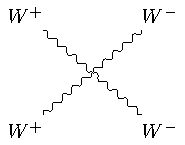
\includegraphics[width=0.3\textwidth]{AnomalousCouplingsTheory/Plots/AGCVertex1.pdf}} 
\subfloat[]{\label{fig:smvertex3}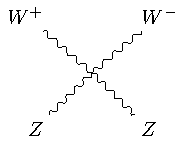
\includegraphics[width=0.3\textwidth]{AnomalousCouplingsTheory/Plots/AGCVertex3.pdf}} 
\subfloat[]{\label{fig:smvertex2}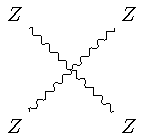
\includegraphics[width=0.3\textwidth]{AnomalousCouplingsTheory/Plots/AGCVertex2.pdf}} 
\caption[Vertices that are sensitive to the anomalous gauge couplings $\alpha_{4}$ and $\alpha_{5}$.]{Vertices that are sensitive to the anomalous gauge couplings $\alpha_{4}$ and $\alpha_{5}$.}
\label{fig:agcvertices}
\end{figure}

The Standard Model already contains triple and quartic vertices involving the electroweak gauge bosons, shown in figure \ref{fig:smtripleandquarticvertices}, which originate from the kinematic terms in the Proca action $\mathcal{L}_{kin} = -\frac{1}{4}B_{\mu\nu}B^{\mu\nu} - \frac{1}{4}W_{\mu\nu}W^{\mu\nu}$.  These vertices are also present in this EFT approach.   

% Feynam diagrams of triple and quartic vertices in the standard model.
\begin{figure}[h!]
\subfloat[]{\label{fig:smvertex1}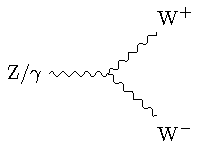
\includegraphics[width=0.3\textwidth]{PhysicsAnalysis/Plots/FeynmanDiagrams/SMVertex1.pdf}} 
\subfloat[]{\label{fig:smvertex2}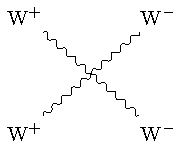
\includegraphics[width=0.3\textwidth]{PhysicsAnalysis/Plots/FeynmanDiagrams/SMVertex2.pdf}} 
\subfloat[]{\label{fig:smvertex3}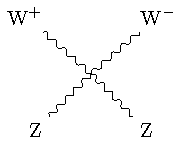
\includegraphics[width=0.3\textwidth]{PhysicsAnalysis/Plots/FeynmanDiagrams/SMVertex3.pdf}} \hfill
\subfloat[]{\label{fig:smvertex4}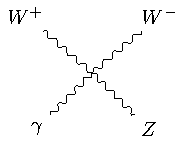
\includegraphics[width=0.3\textwidth]{PhysicsAnalysis/Plots/FeynmanDiagrams/SMVertex4.pdf}} 
\subfloat[]{\label{fig:smvertex5}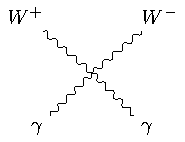
\includegraphics[width=0.3\textwidth]{PhysicsAnalysis/Plots/FeynmanDiagrams/SMVertex5.pdf}} 
\caption[Gauge boson self-coupling vertices in the standard model.]{Gauge boson self-coupling vertices in the standard model.}
\label{fig:smtripleandquarticvertices}
\end{figure}

A study into the sensitivity of the CLIC experiment to the anomalous gauge couplings $\alpha_{4}$ and $\alpha_{5}$ is presented in section \ref{chap:PhysicsAnalysis}.

%========================================================================================
